\documentclass[fleqn]{article}

\usepackage{graphicx}
\usepackage{hyperref}
\usepackage{amsmath}

\title{Information Theory - Midterm}
\author{Zohreh Sadeghi \thanks{University of Washington - Tacoma}}
\begin{document}

\maketitle

\clearpage

\tableofcontents

\clearpage

The code for this project can be found at \url{https://github.com/zsadeghi/info-theory-midterm}.

\section{Question 1: Entropy}

The code provides entropy values for arbitrary n-grams from the text.

Here are the results for uni-grams through 9-grams:

\begin{itemize}
  \item[1-gram] $2.9026942563927163$
  \item[2-gram] $2.498656282450236$
  \item[3-gram] $2.1573949768342944$
  \item[4-gram] $1.7407052326538353$
  \item[5-gram] $1.2607405525003155$
  \item[6-gram] $0.8328141346993452$
  \item[7-gram] $0.5178101859212683$
  \item[8-gram] $0.3069581410914994$
  \item[9-gram] $0.1775738447828046$
\end{itemize}

To put this into a chart, we have:


\begin{figure}[h]
  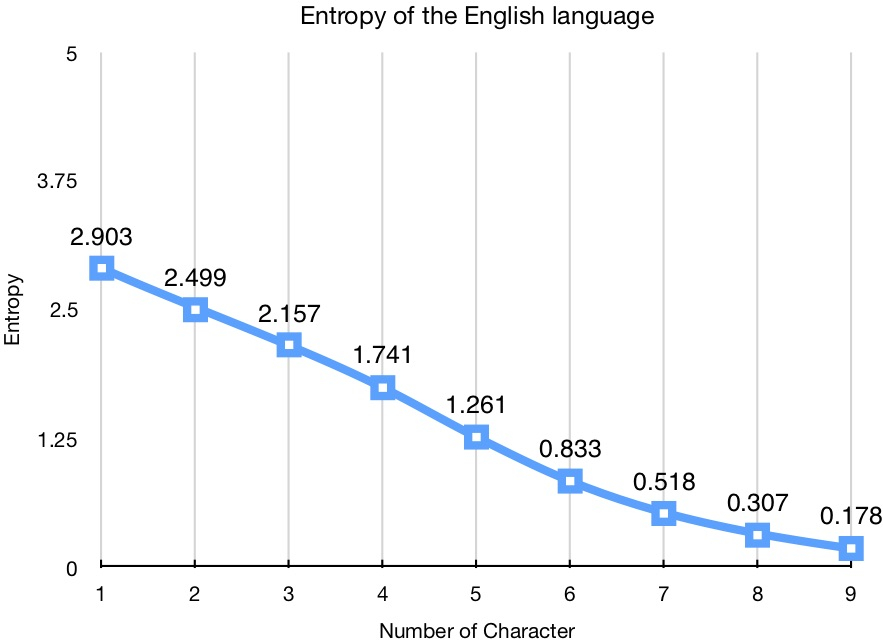
\includegraphics[width=\textwidth]{images/entropy.jpg}
\end{figure}

\clearpage

\section{Question 2: Huffman Coding}

When encoding using single characters, we get the following:

\begin{itemize}
  \item \textbf{Ratio}: $0.3225$
  \item \textbf{Inverted ratio}: $3.1007$
  \item \textbf{Compression time}: 611 milliseconds
  \item \textbf{Decompression time}: 189 milliseconds
\end{itemize}

Using bigrams, we get:

\begin{itemize}
  \item \textbf{Ratio}: $0.3731$
  \item \textbf{Inverted ratio}: $2.6802$
  \item \textbf{Compression time}: 253 milliseconds
  \item \textbf{Decompression time}: 144 milliseconds
\end{itemize}

Using trigrams, we get:

\begin{itemize}
  \item \textbf{Ratio}: $0.4347$
  \item \textbf{Inverted ratio}: $2.3004$
  \item \textbf{Compression time}: 334 milliseconds
  \item \textbf{Decompression time}: 269 milliseconds
\end{itemize}

The inverse of the compression ration seems to be bound by the entropy of the
text from the lower side. In other words, the entropy seems to act as a lower
bound for the inverse of the compression ratio.

\section{Question 3: Structured Tree Lempel-Ziv}

When encoding using single characters as unit of lookup, we get the following:

\begin{itemize}
  \item \textbf{Ratio}: $0.2659$
  \item \textbf{Inverted ratio}: $3.7608$
  \item \textbf{Compression time}: 739 milliseconds
  \item \textbf{Decompression time}: 284 milliseconds
\end{itemize}


\section{Question 4}

\paragraph{a.}
Two series with a length of 3 have a probability of $2^{-3}$.

Therefore:

\begin{align*}
  &2 {3 \choose 1}=6 : \text{ series with length 4}\\
  &p=2^{-4}
\end{align*}

also:

\begin{align*}
  &2 {4 \choose 2}=12 : \text{ series with length 5}\\
  &p=2^{-5}
\end{align*}

From these we can write:

\begin{align*}
  H(X)&=2\times{}2^{-3}\log_2{2^3}+6\times{}2^{-4}\log_2{2^4}
  +12\times{}2^{-5}\log_2{2^5}\\
  &=\frac{33}{8}\\
  &=4.125
\end{align*}

and

\begin{align*}
  H(Y)&=\frac{1}{4}\log_2{4}+2\times{}\frac{3}{8}\log_2{\frac{8}{3}}\\
      &=\frac{1}{2}+\frac{3}{4}\log_2{\frac{8}{3}}\\
      &=1.62
\end{align*}

$Y$ is a deterministic function of $X$, therefore $H(Y|X)=0$.

\begin{align*}
  I(X;Y)=H(Y)=\frac{1}{2} + \frac{3}{2} \log_2{\frac{8}{3}}=1.71
\end{align*}
\begin{align*}
  H(X|Y)=H(X)-H(Y)=\frac{21}{8}-\frac{3}{4}\log_2{\frac{8}{3}}=2.61
\end{align*}
\begin{align*}
  \Rightarrow D(\rho_A||X)=1 \text{ because $\rho_A$ is twice $X$}
\end{align*}
\begin{align*}
  \Rightarrow D(q_A||X)=1 \text{ because $Y$ is independent of $A$ winning the series.}
\end{align*}

Therefore, since this is a win, $q_A$ has the same distribution as $Y$.

\paragraph{b.}

Given that $H(y|z)=H(y)$ and that Shannon's entropy is a nonnegative value,
using the chain rule we have:

\begin{align*}
  H(x,y,z)=H(x|y,z) + H(y|z) \geq H(y|z) + H(z) = H(y) + H(z) = 2
\end{align*}

\section{Question 5}

Zipf's law states that ``given a large sample of words used, the
frequency of any word is inversely proportional to its rank in the frequency
table. So word number $N$ has a frequency of $N$.''.

Now, let's try to calculate the entropy:

\[
  P(n) = \left\{\begin{array}{lr}
      \frac{0.1}{n} & \text{for } n\leq 12367\\
      0 & \text{otherwise }
      \end{array}\right.
\]

Given that Shannon's information content function is

\begin{align*}
  h(x)=-\log{p(x)}
\end{align*}

the entropy could be calculated as the expected value of this function per word:

\begin{align*}
  H(X)=\sum{p(x)\times{}h(p(x))}
\end{align*}

For all the words for which the probability is non-zero, we can write:

\begin{align*}
  H(X)=\frac{\sum_1^{12368}p(n)\times{}h(p(n))}{\log{2}} \approx 9.716 \text{bits per word}
\end{align*}

By comparing the result with my calculations from question 1, we can conclude that
Zipf's law does not yield an accurate function for calculating the entropy of the English
language, as there is quite a few bits of difference in the two results.

\end{document}
